\documentclass[9pt]{article}
\usepackage{fullpage}
\usepackage{amsmath}
\usepackage{amssymb}
\usepackage{graphics}
\usepackage[usenames]{color}
\usepackage{hyperref}
\usepackage{graphicx,wrapfig}
\usepackage{wallpaper}
\usepackage[inline]{enumitem}

\newcommand{\addphoto}[2]{%
  \smash{%
    \makebox[0pt][l]{%
      \raisebox{#1mm}{%
        \hspace{#2mm}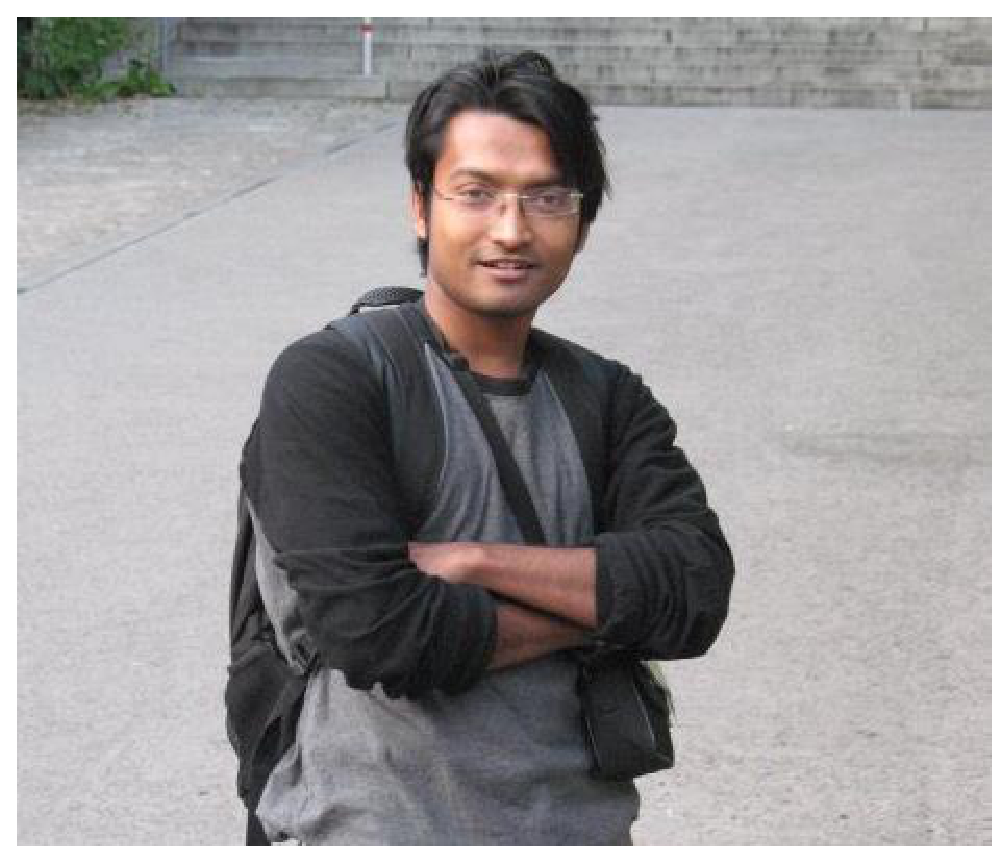
\includegraphics[scale=1]{mypic_1}%
      }%
     }%
  }%
}
\hypersetup{
    colorlinks=true,
    citecolor=blue,%
    filecolor=blue,%
    linkcolor=blue,%
    urlcolor=blue
}


\leftmargin=0.25in
\oddsidemargin=0.25in
\textwidth=6.0in
\topmargin=-0.25in
\textheight=9.25in
\newcommand{\p}{p{8cm}}

\raggedright

\pagenumbering{arabic}

\def\bull{\vrule height 0.8ex width .7ex depth -.1ex }
% DEFINITIONS FOR RESUME

\newenvironment{changemargin}[2]{%
  \begin{list}{}{%
    \setlength{\topsep}{0pt}%
    \setlength{\leftmargin}{#1}%
    \setlength{\rightmargin}{#2}%
    \setlength{\listparindent}{\parindent}%
    \setlength{\itemindent}{\parindent}%
    \setlength{\parsep}{\parskip}%
  }%
  \item[]}{\end{list}
}

\newcommand{\lineover}{
	\begin{changemargin}{-0.05in}{-0.05in}
		\vspace*{-8pt}
		\hrulefill \\
		\vspace*{-2pt}
	\end{changemargin}
}

\newcommand{\header}[1]{
	\begin{changemargin}{-0.5in}{-0.5in}
		\scshape{#1}\\
  	\lineover
	\end{changemargin}
}

\newcommand{\cmnt}[1]{}

\newcommand{\contact}[4]{
	\begin{changemargin}{-0.5in}{-0.5in}
		\begin{center}
			{\Large \scshape {#1}}\\ \smallskip
			{#2}\\ \smallskip 
			{#3}\\ \smallskip
			{#4}\smallskip
		\end{center}
	\end{changemargin}
}

\newenvironment{body} {
	\vspace*{-16pt}
	\begin{changemargin}{-0.25in}{-0.5in}
  }	
	{\end{changemargin}
}	

\newcommand{\school}[4]{
	\textbf{#1} \hfill \emph{#2\\}
	#3\\ 
	#4\\
}

\makeatletter
\newcommand{\inlineitem}[1][]{%
\ifnum\enit@type=\tw@
    {\descriptionlabel{#1}}
  \hspace{\labelsep}
\else
  \ifnum\enit@type=\z@
       \refstepcounter{\@listctr}\fi
    \quad\@itemlabel\hspace{\labelsep}
\fi}        
\makeatother

        
% END RESUME DEFINITIONS

\begin{document}

%%%%%%%%%%%%%%%%%%%%%%%%%%%%%%%%%%%%%%%%%%%%%%%%%%%%%%%%%%%%%%%%%%%%%%%%%%%%%%%%
% Name
	\begin{changemargin}{-0.5in}{-0.5in}
\begin{tabular}{lr}
\begin{tabular}{c}
%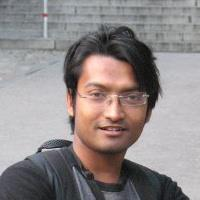
\includegraphics[height=35mm,width=35mm]{mypic3.png}
\includegraphics[width=0.26\textwidth]{mypic5.jpg}
\end{tabular} & 
\begin{tabular}{c}

 {\Large Sandeep Dasgupta} \\ 
\begin{tabular}{l}
\qquad\qquad\qquad\qquad{{\texttt{Email}:\,\,\;\;\, sdasgup3@illinois.edu}} \\
\qquad\qquad\qquad\qquad{{\texttt{Email}:\,\,\;\;\, sandigame.123@gmail.com}} \\
\qquad\qquad\qquad\qquad{{\texttt{Webpage}: \url{http://webhost.engr.illinois.edu/~sdasgup3}}} \\
\qquad\qquad\qquad\qquad{{\texttt{Github}:\;\,  \url{https://github.com/sdasgup3}}} \\
\qquad\qquad\qquad\qquad{{\texttt{Phone}:\;\;\,   (+1) 2174172344}} \\
\end{tabular}  
\end{tabular} \\
&\\
\end{tabular} 

	\end{changemargin}


%%%%%%%%%%%%%%%%%%%%%%%%%%%%%%%%%%%%%%%%%%%%%%%%%%%%%%%%%%%%%%%%%%%%%%%%%%%%%%%%
% Objective
\header{Interested In}
\begin{body}
	\vspace{14pt}
	\begin{itemize} \itemsep -0pt
		\item Compiler (LLVM, GCC) (Frontend/Backend/Optimizations)  \qquad\quad\;\   \inlineitem Binary Code Decompilation
		\item Static/Dynamic Program Analysis   \qquad\qquad\qquad\quad   \inlineitem Language Formal Semantics
                \item Design of Interpreter \& Dynamic typed languages \   \inlineitem Parallel \& Power Aware Computation
                \item  Data Analysis using Statistical tools \qquad\qquad\qquad\ \inlineitem Symbolic Execution
	  \end{itemize}

        \medskip  

	  \textbf{Languages proficient with}\\
	  \begin{itemize} \itemsep -0pt
		\item Go, C++, Swift, Haskel, C, Assembly \inlineitem  Perl, Python, R  \inlineitem Pthread, OpenMP, MPI, Charm++
		%\item Perl, Python
		%\item Pthread, OpenMP, MPI, Charm++
	  \end{itemize}

%		Parallel Computing \\
%		Programming Language Design \& Implementation \\
% 		Automated software verification \& quality assurance.
\end{body}


\smallskip


%%%%%%%%%%%%%%%%%%%%%%%%%%%%%%%%%%%%%%%%%%%%%%%%%%%%%%%%%%%%%%%%%%%%%%%%%%%%%%%%
% Education
\header{Career Overview}

\begin{body}
	\vspace{14pt}

        \textbf{PhD Computer Science -- GPA 3.95/4.00}{} \hfill \emph{Aug'13 - May'20 (Expected)}{} \\
	\textbf{\emph{\href{http://cs.illinois.edu/}{CS @ University of Illinois Urbana Champaign}}{}} \\
	\begin{itemize} \itemsep -0pt
            \item  Working with Prof.
              \href{http://vikram.cs.illinois.edu/}{Vikram S.
              Adve} on \href{https://publish.illinois.edu/allvm-project/}{ALLVM
              Research Project}
          \item  Current Research 
            \begin{itemize} 
              \item Formal semantics of X86-64 ISA. \textbf{\emph{{\href{https://github.com/kframework/X86-64-semantics}{Public Repository}}}}

              \item Validating the decompilation from binary to LLVM IR: Given
              the importance of binary analysis, establishing the faithfulness
              of a binary lifter (or decompiler) is most desirable, and is the
              current focus of my work. Specifically, we are developing
              techniques and tools for the translation validation of binary decompilers to
              LLVM IR, including defining the semantics of LLVM IR and X86-64 ISA,
              which is required for that validation.

            \end{itemize} 
        \end{itemize}

 \medskip

        \textbf{Software Engineering Intern, with Stephane Eranian, Kernel performance team} \hfill \emph{Sept'18 - Dec'18}\\
	\textbf{\emph{\href{https://www.google.com/intl/en/about/}{Google Inc.}}}
	\begin{itemize} \itemsep -0pt


        \item First, Developed from scratch an
        \href{https://ieeexplore.ieee.org/document/6844459}{``Intel Topdown''}
        converter that we will be released to the open-source community. This will
        make the Intel Topdown bottleneck analysis methodology more visible and
        successful.

                        \cmnt{
                \item  Augmented the
                \href{https://git.kernel.org/pub/scm/linux/kernel/git/tip/tip.git/tree/tools/perf}{perf}
                tools with
                \textbf{\emph{\href{https://ieeexplore.ieee.org/document/6844459}{``Topdown
                  Analysis''}}} capability.
			\begin{itemize}
                                \item Intel developed a cycle decomposition
                                methodology called
                                \emph{\href{https://ieeexplore.ieee.org/document/6844459}{Topdown}}.
                                It uses about 60 hardware events to breakdown
                                micro-architectural performance bottlenecks
                                encountered by running software on Intel
                                processors. It is very useful in characterizing
                                workloads and focusing on where to apply
                                optimizations.  Topdown is described as a tree
                                of metrics, each one requiring many events, and
                                published as a complex spreadsheet. The goal of
                                the project is to automate the conversion of
                                the formulas in the spreadsheet into C code
                                that can be integrated into the perf tool.
                                Today, this conversion is done by hand. As the
                                spreadsheet is constantly evolving to support
                                new hardware and tweak of the formulas, we need an
                                automated way of doing the conversion. Such an
                                automated converter is realized in this
                                project.

                                \item We developed tool ‘topdown\_parser’ which
                                takes as input, the topdown xlsx, and generates
                                C code to collect and report all levels of
                                topdown tree across all supported processors.
                                The tool is general enough to emit code
                                (encoding the topdown formulas) for other
                                projects like,
                                \emph{\href{https://git.kernel.org/pub/scm/linux/kernel/git/tip/tip.git/tree/tools/perf}{
                                  Public perf tool}}, in which case we emit
                                  json files encoding the topdown metric
                                  expression.

			\end{itemize}
                        }

\item Second, Developed proof-of-concept prototypes to achieve data profile symbolization.
                %\item Data Profiling to extract type information from binaries:
                Given a set of hot load/store instructions (generated by
                    sampling the application using tools like perf), the
                problem is to find the type of the data address associated with
                those instructions. Such information is useful in optimizing memory
                allocation strategies or cache utilization.  Deployed
                LLVM based tools implementing approaches based on: (1)
                Allocation Based Profiling and (2) Dwarf debug Info.
                \item Received manager's recognition via spot bonus.

                \cmnt{
			\begin{itemize}

                          \item Based on Allocation Based Profiling: We
                          generate samples of allocation information (like
                              allocation base address, size, etc) and use that
                          to find which allocation is feeding a particular
                          load/store data address.

                          \item Based on Dwarf debug Info: Dwarf debug
                          information stores, as a best effort, the variables
                          in a given scope along with its associated type. The
                          idea is to find which variable, in load/store
                          instruction's scope, is getting consumed by a given
                          load/store data address. For that we needed to parse
                          the location list information of dwarf.

			\end{itemize}
                }

	\end{itemize}

        \textbf{Software Engineering Intern, Tipp Moseley, Continuous profiling team} \hfill \emph{May'17 - Aug'17}\\
	\textbf{\emph{\href{https://www.google.com/intl/en/about/}{Google Inc.}}}
	\begin{itemize} \itemsep -0pt
                \item  Augmented the profiling tools with analysis capable of
                guiding the service owners to pinpoint unexpected performance
                changes (called ``havocs'' in this work) in CPU time.

                        \cmnt{Challenges are:
			\begin{itemize}
				\item To determine ``havocs'' amid noisy data.
				\item To reduce false positives and pinpoint actionable ``havocs'' to the service providers.
			\end{itemize}
                        }
		%\item Investigated the effectiveness of existing strategies in literature and open source.
		%\item
			Developed a statistical Go tool which determines
			potential ``havocs'' with reduced false positive rate.
			Came up with an idea of correlating the
			statistically detected trend changes in the data with
			build CL changes which not only gives confidence on
			trend change detection but also helps in reducing the
			false positives.

		%\item Carried out the research part of the project
		%	independently aligning the milestones and the work
		%	progress with the project supervisor. Collaborated with
		%	the team on the details of integrating with the data
		%	querying pipeline.
		%\item Benefited by attending \& socializing @Google's PhD Intern Research Conference, 2017.
		%\item Volunteered @UIUC Alumni Event, 2017.
	\end{itemize}


 \medskip
        \textbf{Compiler Engineer Intern, with Roman Levenstein, Swift performance team} \hfill \emph{April'16 - Aug'16}\\
	\textbf{\emph{\href{http://www.apple.com}{Apple Inc.}}}
	\begin{itemize} \itemsep -0pt

                \item  Achieved functional completeness in converting swift to JS. Involves 
                 converting swift programs to LLVM bitcode using the
                swift compiler infrastructure and then use emscripten to convert the result to
                JS. The challenges include (but not limited to):
                  \begin{itemize}
                    \item Converting Swift standard and runtime library into LLVM IR
                    \item Enhancing emscripten type legalization for small integer types like i3
                    \item Enhancing emscripten address relocations support
                    \item Supporting dynamic loading of JavaScript generated from emscripten
                    \item Adjustments in runtime library  to support Type and protocol conformance metadata
                  \end{itemize}

	\end{itemize}

 \medskip
        \textbf{Component Design Engineer} \hfill \emph{Aug'11 - Jun'13}\\
	\textbf{\emph{\href{http://www.intel.in/content/www/in/en/homepage.html}{Intel Technology India Pvt. Ltd.}}}
	\begin{itemize} \itemsep -0pt
                \item Worked as Design Automation Engineer for Formal Equivalence Verification (FEV) of hardware designs for Broadwell (BDX) and Skylake (SKL) projects. Involves
                building flows and methodologies and interacting closely with
                global FEV teams to provide FEV solutions.
                \item Owner of tools and infrastructures for driving
                FEV central runs for  BDX. Invloves working closely with teams of various
                design styles.
	\end{itemize} 

 \medskip
	\textbf{M.Tech Computer Science \& Engineering -- CPI 9.00/10.00}{} \hfill \emph{Aug'09 - Jun'11}{} \\
	\textbf{\emph{\href{http://www.iitk.ac.in/}{Indian Institute Of Technology Kanpur}, Kanpur, India.}{}} \\
	\begin{itemize} \itemsep -0pt
		\item Secured \textbf{rank} $1$ in M. Tech 2009 Batch, IIT Kanpur.
	\end{itemize}

 \medskip
        \textbf{Senior Member Of Technical Staff} \hfill \emph{Aug'06 - Jul'09}\\
       	\textbf{\emph{\href{http://www.interrasystems.com/}{Interra Systems India Pvt. Ltd.}}}
	\begin{itemize} \itemsep -0pt
		\item Developer of Interra's premiere front-end analyzer products - Cheetah (SystemVerilog) and MVV(Mixed Verilog Vhdl) and 
		provided support for several new constructs of System Verilog IEEE-1800-2005. 
		\item Worked with \href{http://www.atrenta.com/}{Atrenta (I) Pvt. Ltd.} (service project) for the development of System Verilog features in Spyglass DFT.
		\item Awarded \textbf{Interra Humming Bird Award} in recognition of \& appreciation for providing excellent support to \href{}{Atrenta (I) Pvt. Ltd.} in the project ``IEEE compliance for Spyglass''.
	\end{itemize}

  \medskip
	\textbf{B.E. Computer Science \& Engineering -- \emph{First Class with Honors}, 85.625/100.00} \hfill \emph{Aug'02 - Jun'06} \\
	\textbf{\emph{\href{http://www.iiests.ac.in/}{Indian Institutes of Engineering Science and Technology, Shibpur}}, West Bengal, India.}\\
	\begin{itemize} \itemsep -0pt
		\item Awarded \textbf{University Gold Medal} for securing 1st Rank in BE, Computer Science \& Engineering, '02 batch.
		\item Awarded \textbf{Best Student Award}, sponsored by \href{http://www.tcs.com}{Tata Consultancy Services}, for outstanding performance in BE, Computer Science \& Engineering, 2002 batch.
	\end{itemize}
\end{body}

\smallskip

%%%%%%%%%%%%%%%%%%%%%%%%%%%%%%%%%%%%%%%%%%%%%%%%%%%%%%%%%%%%%%%%%%%%%%%%%%%%%%%%
% Publications
\header{Publications}
\begin{body}
\vspace{14pt}
\textbf{Conferences}\\
	\vspace*{-4pt}
	\begin{itemize} \itemsep -0pt
		\item \underline{Sandeep Dasgupta}, Daejun Park, Theodoros Kasampalis, Vikram S. Adve  \& Grigore Rosu.``\textbf{A Complete Formal Semantics of x86-64 User-Level
Instruction Set Architecture}'', in \emph{Programming Language Design and Implementation}, PLDI 2019. \\
                \href{http://webhost.engr.illinois.edu/~sdasgup3/Document/pldi_2019.pdf}{[PDF]}
                \href{https://dl.acm.org/citation.cfm?id=3314221.3314601}{[DOI]}
                \href{http://webhost.engr.illinois.edu/~sdasgup3/Document/pldi_2019.bib}{[BIB]}
                \href{https://conf.researchr.org/home/pldi-2019}{[PLDI'19]}

		\item \underline{Sandeep Dasgupta} \& Amey Karkare.``\textbf{Precise shape analysis using field sensitivity}'', in \emph{Proceedings of the 27th Annual ACM Symposium on Applied Computing}, SAC 2012. \\
                \href{http://webhost.engr.illinois.edu/~sdasgup3/Document/sac_2012.pdf}{[PDF]}
                \href{http://dx.doi.org/10.1145/2245276.2231982}{[DOI]}
                \href{http://webhost.engr.illinois.edu/~sdasgup3/Document/sac_2012.bib}{[BIB]}
                \href{https://www.sigapp.org/sac/sac2012/}{[SAC'12]}

		\item Barnali Basak, \underline{Sandeep Dasgupta} \& Amey Karkare.``\textbf{Heap Dependence Analysis for Sequential Programs}'', \emph{International Conference on Parallel Computing}, ParCo 2011. \\ 
                \href{http://webhost.engr.illinois.edu/~sdasgup3/Document/parco_2011.pdf}{[PDF]}
                \href{http://dx.doi.org/10.3233/978-1-61499-041-3-99}{[DOI]}
                \href{http://webhost.engr.illinois.edu/~sdasgup3/Document/parco_2011.bib}{[BIB]}
                \href{http://parco2011.elis.ugent.be/}{[ParCo'11]}
	\end{itemize}

\textbf{Journals \& Workshops}\\
\vspace{-4pt}
\begin{itemize} \itemsep -0pt
     \item  Andrew H. Miranti, \underline{Sandeep Dasgupta}. ``\textbf{Formalizing x86-64 Instruction Decoder in K}, in \emph{Workshop on Instruction Set Architecture Specification}, SpISA 2019. \\
     \href{http://webhost.engr.illinois.edu/~sdasgup3/Document/spisa_2019.pdf}{[PDF]}
     \href{https://www.cl.cam.ac.uk/~jrh13/spisa19.html}{[SpISA'19]}

    \item \underline{Sandeep Dasgupta}, Amey Karkare \& P.\ Vinay K.\ Reddy. ``\textbf{Precise shape analysis using field sensitivity}.'', in \emph{Innovations in Systems and Software Engineering}, ISSE 2013. \\
    \href{http://webhost.engr.illinois.edu/~sdasgup3/Document/isse_2013.pdf}{[PDF]}
    \href{http://www.springerlink.com/openurl.asp?genre=article&id=doi:10.1007/s11334-013-0198-7}{[DOI]}
    \href{http://webhost.engr.illinois.edu/~sdasgup3/Document/isse_2013.bib}{[BIB]}
    \href{https://link.springer.com/journal/11334}{[ISSE'13]}
\end{itemize}

\textbf{Invited Talks}\\
\vspace{-4pt}
\begin{itemize} \itemsep -0pt
    \item  \underline{Sandeep Dasgupta}. ``\textbf{The K Framework}.'', in \emph{Workshop on Declarative Program Analysis}, DPA 2019. \\
    \href{http://webhost.engr.illinois.edu/~sdasgup3/Document/dpa_2019.pdf}{[PDF]}
    \href{https://pldi19.sigplan.org/details/dpa-2019-papers/5/The-K-Framework}{[DPA'19]}
\end{itemize}

\textbf{Poster Submissions}\\
	\vspace*{-4pt}
	\begin{itemize} \itemsep -0pt
                \item \underline{Sandeep Dasgupta} and Vikram S. Adve. ``\textbf{A Complete Formal Semantics of User-Level ISA}.'', in \emph{Office of Naval Research (ONR), Total Platform Cyber Protection Program Meet}, 2019. \\
  		\href{http://webhost.engr.illinois.edu/~sdasgup3/Document/onr-tpcp-19.pdf}{[PDF]}

                \item \underline{Sandeep Dasgupta}, Joshua Cranmer, Edward Schwartz and Vikram S. Adve. ``\textbf{Binary Decompilation to LLVM IR
                  }'', LLVM Developers' Meeting, 2016. \\
                  \href{http://webhost.engr.illinois.edu/~sdasgup3/Document/allin_poster.pdf}{[PDF]}
                  \href{https://llvm.org/devmtg/2016-11/}{[LLVM Dev Meet'16]}

                \item \underline{Sandeep Dasgupta}, Barnali Basak \& Amey Karkare. ``\textbf{Dependence Analysis for Parallelization of Sequential Programs}'', the 8th ASIAN
                  Symposium on Programming Languages \& Systems, APLAS 2010. \\
                  \href{http://webhost.engr.illinois.edu/~sdasgup3/Document/poster_APLAS2010.pdf}{[PDF]}
                  \href{https://basics.sjtu.edu.cn/conference/aplas2010/accepted_posters.htm}{[APLAS'10]}
	\end{itemize}


\end{body}

\smallskip

%%%%%%%%%%%%%%%%%%%%%%%%%%%%%%%%%%%%%%%%%%%%%%%%%%%%%%%%%%%%%%%%%%%%%%%%%%%%%%%%
% Courses and Projects
%\newpage
\header{Other Projects \& Services}

\begin{body}
	\vspace{14pt}
	\textbf{Projects}{} \hfill  \\
	\begin{itemize} \itemsep 3pt

           \item \textbf{x86-64 Instruction Semantics}
           \href{https://github.com/StanfordPL/stoke/pulls?q=is%3Apr+author%3Asdasgup3+is%3Aclosed}{[Pull requests on Stoke]} \\ 
           \texttt{Abstract: } Porting my work on most complete x86-64 instruction semantics (Dasgupta et al., PLDI'19) to an
open source x86 superoptimizer tool, Stoke, inorder to benefit downstream tools built on top of it.


           \item \textbf{Profiler Using \emph{Clang} based AST Instrumentation}
           \href{https://github.com/sdasgup3/profiler-using-clang-based-ast-instrumentation}{[Github]} \\ 
           \texttt{Abstract: } \emph{Clang} based AST reformatting tool used for
           injecting instrumentation code in C/C++ programs. The goal is
           collecting profiles (run-times and execution frequencies) on C/C++
           programs.

           \item \textbf{\emph{LLVM} based Dwarf Type Reader} 
           \href{https://github.com/sdasgup3/dwarf-type-reader}{[Github]} \\
             \texttt{Abstract: } To read type information from \emph{debug info}
             section of executables using \emph{LLVM} based APIs.

           \item \textbf{Decompiling binary to ``rich'' LLVM IR}
           \href{https://github.com/sdasgup3/binary-decompilation/blob/master/libs/stack_deconstructor/stack_deconstructor.cpp}{[Github]} \\ 

\texttt{Abstract: } One of the limitations of existing binary-to-LLVM IR
decompilers is that the extracted IR misses high level informations like
variables and types. Moreover, some of them uses a flat array to model the
runtime process stack which is shared by all the procedures. This inhibits many
aggressive optimizations on the modeled stack because of potential aliases
between procedures.  Towards our goal of extracting richer LLVM IR from binary,
        we have implemented the following IR transformation passes on the
        decompiled LLVM IR: (1) Distinguish individual stack frames, and (2)
        Identify local variables in each stack frame.

           \item \textbf{Pointer Analysis Debugger} 
             %\href{http://webhost.engr.illinois.edu/~sdasgup3/Document/pa_debugger.pdf}{[Presentation]} 
             \href{https://www.dropbox.com/s/pm47zniafdydotw/pa_debugger.pdf?dl=0}{[Presentation]} 
           \href{https://github.com/sdasgup3/symbolic-analysis}{[Github]} \\
                                  \texttt{Abstract: } To detect bugs in LLVM's
                                  pointer analysis using a mix of static
                                  program analysis and dynamic symbolic
                                  execution. 

           \item \textbf{Partial Redundancy Elimination(PRE)} 
           \href{http://webhost.engr.illinois.edu/~sdasgup3/Document/report_cs526.pdf}{[Report]} 
           \href{https://github.com/sdasgup3/partial-redundancy-elimination}{[Github]} \\
                                  \texttt{Abstract: } Implemented a PRE
                                  optimization pass in LLVM and measured results
                                  on a variety of applications and did a detailed 
                                  study on the performance numbers. 

            \item \textbf{Extended GCC's Global Dataflow Analyzer} 
           \href{http://webhost.engr.illinois.edu/~sdasgup3/Document/report_gdfa.pdf}{[Report]} 
           \href{https://github.com/sdasgup3/non-separable-global-dataflow-framework}{[Github]} \\
                                \texttt{Abstract: }Extended the Generic Data Flow Analyzer
                                GDFA (of gcc) to the data flow frameworks where
                                data flow information can be represented using
                                bit vectors but the frameworks are not bit
                                vector frameworks because they are
                                non-separable e.g., faint variable analysis,
                                possible undefined variable analysis, strongly
                                live variable analysis.	

           \item \textbf{Designing an Interpreter of a dynamic language for Graph
algorithms}
           \href{http://webhost.engr.illinois.edu/~sdasgup3/Document/report_cs598dhp.pdf}{[Report]} 
           \href{https://github.com/sdasgup3/gri}{[Github]} \\
                                  \texttt{Abstract: } 
                                  Designed a dynamically typed language and an interpreter for it and 
                                  achieved a slowdown of 2X w.r.t the execution time of statically compiled C
                                  language. This is obtained by providing built-in compiled functions 
                                  for simple graph computation which in turn help to build complex
                                  ones.

          \item \textbf{Mitigating Impact of Heterogeneity Across Power-constrained Nodes on Parallel Applications through Load Balancing}     
                                \href{http://webhost.engr.illinois.edu/~sdasgup3/Document/report_cs533.pdf}{[Report]} 
                                \href{https://github.com/sdasgup3/heterogeneity-aware-load-balancing}{[Github]} \\
                                  \texttt{Abstract: }Different processors across the nodes
                                  have different execution times for the same
                                  work-loads. This performance imbalance is seen
                                  only when the CPU power is capped to low
                                  values. This performance imbalance causes
                                  increased execution times of the parallel
                                  applications. We did a detailed study and
                                  proposed a power aware load balancer (using
                                      Charm++ ) which minimized the performance
                                  imbalance at the lower power caps by tackling
                                  this heterogeneity.  
           \item \textbf{Designing superscalar processor} \href{https://github.com/sdasgup3/parallel-processor-design}{[Github]} \\
                                \texttt{Abstract: } Developed a superscalar processor (with  an
                                    issue rate of 2) using verilog hdl, and an
                                assembler for that processor using flex and
                                bison.  

           \item \textbf{Graph Coloring Using State Space Search} 
           \href{http://webhost.engr.illinois.edu/~sdasgup3/Document/CS598_project_proposal.pdf}{[Report]} 
           \href{https://github.com/sdasgup3/parallel-sudoku}{[Github]} \\          
                                  \texttt{Abstract: }Leveraged the state space
                                  search model for implementing graph coloring
                                  in parallel in Charm++. Some of the
                                  challenges for efficient exploration of space
                                  by chares include intelligent pruning of the
                                  state space, load balancing, grain-size
                                  control and low-overhead communication
                                  between chares. Evaluated multiple options
                                  for each of these, and come up with design
                                  decisions which would work for a large
                                  category of real-life graph applications.
	\end{itemize}
	\textbf{Services}{} \hfill  \\

	\begin{itemize} \itemsep 3pt
          \item Sub-reviewer, The 30th International Conference on Concurrency Theory \href{https://event.cwi.nl/concur2019/}{[CONCUR 2019]}
          \item Sub-reviewer, Workshop on Instruction Set Architecture Specification \href{https://www.cl.cam.ac.uk/~jrh13/spisa19.html}{[SpISA 2019]}
	\end{itemize}
\end{body}

\smallskip

%%%%%%%%%%%%%%%%%%%%%%%%%%%%%%%%%%%%%%%%%%%%%%%%%%%%%%%%%%%%%%%%%%%%%%%%%%%%%%%%
%Professional Experience
\cmnt{
\header{Professional Experience}

\begin{body}
	\vspace{14pt}
	\href{https://www.google.com/intl/en/about/}{\textbf{Google Inc.}}, \emph{Software Engineering Engineer} \hfill \emph{May 2017 - August 2017}\\
	\vspace*{-4pt}
	\begin{itemize} \itemsep -0pt
		\item  Worked in ``Google continuous profiling and efficiency'' team to augment the
			profiling tools with analysis capable of
			guiding the service owners to pinpoint unexpected
			performance changes (called ``havocs'' in this work) in CPU time. Challenges are:
			\begin{itemize}
				\item To determine ``havocs'' amid noisy data.
				\item To reduce false positives and pinpoint actionable ``havocs'' to the service providers.
			\end{itemize}
		\item Investigated the effectiveness of existing strategies in literature and open source.
		\item
			Developed a statistical Go tool which determines
			potential ``havocs'' with reduced false positive rate.
			Came up with an idea of correlating the
			statistically detected trend changes in the data with
			build CL changes which not only gives confidence on
			trend change detection but also helps in reducing the
			false positives.

		\item Carried out the research part of the project
			independently aligning the milestones and the work
			progress with the project supervisor. Collaborated with
			the team on the details of integrating with the data
			querying pipeline.
		\item Benefited by attending \& socializing @Google's PhD Intern Research Conference, 2017.
		\item Volunteered @UIUC Alumni Event, 2017.
	\end{itemize}

	\vspace*{-4pt}
	\href{http://www.apple.com}{\textbf{Apple Inc.}}, \emph{Compiler Engineer, PhD Intern} \hfill \emph{April 2016 - August 2016}\\
	\vspace*{-4pt}
	\begin{itemize} \itemsep -0pt  % reduce space between items
                \item  Worked as a member of Swift Performance Team on an
                  exploratory project which requires sound knowledge in
                  compiler backend. Achieved functional completeness with real
                  work loads.
                \end{itemize}

	\href{http://www.intel.in/content/www/in/en/homepage.html}{\textbf{Intel Technology India Pvt. Ltd.}}, \emph{Component Design Engineer} \hfill \emph{August 2011 - June 2013}\\
	\vspace*{-4pt}
	\begin{itemize} \itemsep -0pt  % reduce space between items
                \item Worked as Design Automation Engineer for Formal Equivalence Verification (FEV) of hardware designs for Broadwell (BDX) and Skylake (SKL) projects. Involves
                building flows and methodologies and interacting closely with
                global FEV teams to provide FEV solutions.
                \item Owner of tools and infrastructures for driving
                FEV central runs for  BDX. Invloves working closely with teams of various
                design styles.
                \end{itemize}

	\href{http://www.interrasystems.com/}{\textbf {Interra Systems India Pvt. Ltd.}}, \emph{Senior Member Of Technical Staff} \hfill \emph{August 2006 - July 2009}\\
	\vspace*{-4pt}
	\begin{itemize} \itemsep -0pt
		\item Developer of Interra's premiere front-end analyzer products - Cheetah (SystemVerilog) and MVV(Mixed Verilog Vhdl) and 
		provided support for several new constructs of System Verilog IEEE-1800-2005. 
		\item Worked with \href{http://www.atrenta.com/}{Atrenta (I) Pvt. Ltd.} (service project) for the development of System Verilog features in Spyglass DFT.
		\item Awarded \textbf{Interra Humming Bird Award} in recognition of \& appreciation for providing excellent support to \href{}{Atrenta (I) Pvt. Ltd.} in the project ``IEEE compliance for Spyglass''.
	\end{itemize}
\end{body}
}

\smallskip

%%%%%%%%%%%%%%%%%%%%%%%%%%%%%%%%%%%%%%%%%%%%%%%%%%%%%%%%%%%%%%%%%%%%%%%%%%%%%%%%
%Hobbies 
\header{My Hobbies}

\begin{body}
	\vspace{14pt}

	\href{https://en.wikipedia.org/wiki/Kuk\_Sool\_Won}{\textbf{Kuk Sool Won}}\\
	\vspace*{-4pt}
	\begin{itemize} \itemsep -0pt  % reduce space between items
                \item  

                  At the moment I am actively learning "Kuk Sool Won", a Korean
                  martial arts system, which involves systematic study of all
                  traditional fighting arts. This incorporates physical
                  exercise, as well as mental development and traditional
                  weapons training.
                  
                \end{itemize}

	\textbf{Dancing}\\
	\vspace*{-4pt}
	\begin{itemize} \itemsep -0pt  % reduce space between items
            \item I am also fond of dancing and choreography, preferably on \href{https://en.wikipedia.org/wiki/Bollywood}{Bollywood} Beats. Have a look
	        \begin{itemize} \itemsep -0pt  % reduce space between items
                    \item \href{https://www.youtube.com/watch?v=jx-HcAEbJaw&feature=youtu.be}{Group@UIUC Durga Puja Festival 2016}
                    \item \href{https://www.youtube.com/watch?v=PfqsE7sajm8&feature=youtu.be}{Group@UIUC Tagore Festival 2016}
                    \item \href{https://www.youtube.com/watch?v=XG6ViBPG7yE}{Solo@UIUC New Year Festival 2015}
                    \item \href{https://www.youtube.com/watch?v=F8xdb7LkSrw}{Solo@IIT Kanpur, Hall Festival 2011}
                \end{itemize}
         \end{itemize}

	\textbf{Table Tennis}\\
	\vspace*{-4pt}
	\begin{itemize} \itemsep -0pt  % reduce space between items
                \item  
                  I have spent considerable amount of time playing Table Tennis
                  with excellent players, so ping pong comes naturally  to me.
                \end{itemize}
\end{body}

\smallskip
%%%%%%%%%%%%%%%%%%%%%%%%%%%%%%%%%%%%%%%%%%%%%%%%%%%%%%%%%%%%%%%%%%%%%%%%%%%%%%%%
\cmnt{
%Teaching Experience
\header{Teaching Experience}

\begin{body}
	\vspace{14pt}
	\textbf{University Of Illinois Urbana Champaign},  \hfill \emph{August 2013 - December 2013}\\
	\vspace*{-4pt}
	\begin{itemize} \itemsep -0pt  % reduce space between items
		\item \textbf{Teaching Assistant} for \href{http://cs.illinois.edu/courses/profile/CS427-120138}{CS 427: Software Engineering I}: A Graduate level course.
			\begin{itemize}
				\item Designing the questions for homework and term examinations and grading those.
				\item Conducting discussion sessions with the students to answer questions related to lectures/homework.   
			\end{itemize}
	\end{itemize}

	\textbf{Indian Institute of Technology, Kanpur},  \hfill \emph{August 2009 - 2011}\\
	\vspace*{-4pt}
	\begin{itemize} \itemsep -0pt  % reduce space between items
		\item \textbf{Tutor} for \href{http://www.cse.iitk.ac.in/teaching/courses/ESc101.html}{ESc 101: Fundamentals of Computing}: An undergraduate course.
			\begin{itemize}
				\item Responsible for weekly lecture class on C - programming language, supervision of programming laboratory and grading assignments and term examinations.
			\end{itemize}
		\item \textbf{Teaching Assistant} for \href{http://www.cse.iitk.ac.in/teaching/courses/CS335.html}{CS 335: Principles of Compiler Design}: An undergraduate course.
			\begin{itemize}
				\item Responsible for mentoring a student group on a course project of developing a simple compiler (using a subset of C-language constructs) demonstrating most of the phases of compiler design starting from Lexical \& Syntax analysis upto Intermediate code generation.
				\item Grading assignments and term examinations.
			\end{itemize}
		\item \textbf{Teaching Assistant} for \href{http://www.cse.iitk.ac.in/teaching/courses/CS355.html}{CS355: Programming Tools and Techniques}: An undergraduate course.
			\begin{itemize}
				\item Grading assignments related to Software management tools such as make; Programming tools such as Python, Perl; Document preparation systems such as tex; Tools for building programs like Lex and Yacc.
			\end{itemize}
	\end{itemize}
\end{body}

\smallskip
}
%%%%%%%%%%%%%%%%%%%%%%%%%%%%%%%%%%%%%%%%%%%%%%%%%%%%%%%%%%%%%%%%%%%%%%%%%%%%%%%%
\cmnt{
% Awards and Honors
\header{Achievements/Distinctions}

\begin{body}
	\vspace{14pt}
	\begin{itemize} \itemsep -0pt  % reduce space between items
	%	\item Awarded \textbf{University Gold Medal} for securing 1st Rank in BE, Computer Science \& Engineering, 2002 batch.\\
	%	\item Awarded \textbf{Best Student Award}, sponsored by \href{http://www.tcs.com}{Tata Consultancy Services}, for outstanding performance in BE, Computer Science \& Engineering, 2002 batch. \\
	%	\item \textbf{Secured Rank $1$}, in M. Tech 2009 Batch, IIT Kanpur.
	%	\item \textbf{Secured All India Rank $145$} (99.64 percentile) in GATE 2009, an exam for admission in Graduate Study.
	%	\item \textbf{Ranked $356^{th}$} (among $\frac{1}{10}$ of Million+ students) in WB-JEE, 2002, an exam for admission in undergraduate study.
	\end{itemize} 
\end{body}

\smallskip
}



\end{document}


\cmnt{
%%%%%%%%%%%%%%%%%%%%%%%%%%%%%%%%%%%%%%%%%%%%%%%%%%%%%%%%%%%%%%%%%%%%%%%%%%%%%%%%
% MTech Course Projects
\header{M.Tech Course Projects}

\begin{body}
	\vspace{14pt}
	\textbf{\href{http://www.cse.iitk.ac.in/teaching/courses/CS738.html}{Advanced Compiler Optimizations}} \\
		\begin{itemize} \itemsep -0pt 
			\item[] To Extend the Generic Data Flow Analyzer GDFA (of gcc) to the data flow frameworks where data flow information can
				be represented using bit vectors but the frameworks are not bit vector frameworks because they are non-separable e.g.,
				faint variable analysis, possible undefined variable analysis, strongly live variable analysis.
		\end{itemize}

  		\medskip

	\textbf{\href{http://www.cse.iitk.ac.in/teaching/courses/CS633.html}{Parallel Computing}} \\
		\begin{itemize} \itemsep -0pt 
			\item[] To design a customized processor (using parallel processing concepts) for the application of document retrieval
				system. We developed a \href{https://github.com/sdasgup3/parallel-processor-design}{superscalar processor (with  an issue rate of 2)} using verilog hdl, and an assembler for that processor using flex and bison.
		\end{itemize}
\end{body}

\smallskip
%\newpage

%%%%%%%%%%%%%%%%%%%%%%%%%%%%%%%%%%%%%%%%%%%%%%%%%%%%%%%%%%%%%%%%%%%%%%%%%%%%%%%%
% BTech Course Projects
\header{B.Tech Project \hfill under supervision of \href{http://cse.iitkgp.ac.in/~pb}{Dr. Partha Bhowmick}}

\begin{body}
	\vspace{14pt}
	\textbf{\href{http://dl.dropbox.com/u/86719354/BE_project.pdf}{Affine Transformation of Digital Curves Using Chain Codes.}}  \\
		\begin{itemize} \itemsep -0pt  
		\item[]  Affine Transformation of Digital Curves Using Chain Codes. The problem statement is to rotate a digital image by a given angle.
		\end{itemize}
\end{body}

\smallskip
\smallskip

%%%%%%%%%%%%%%%%%%%%%%%%%%%%%%%%%%%%%%%%%%%%%%%%%%%%%%%%%%%%%%%%%%%%%%%%%%%%%%%%
% References
\header{References}
	\vspace{14pt}

\begin{body}
%\begin{table}[position specifier]
%\centering
\begin{tabular}{l|l}

& \\
	\begin{tabular}{\p}
		\href{http://www.cse.iitk.ac.in/users/karkare/}{Dr. Amey Karkare}, \\
		Assistant Professor, \\
		Department Of Computer Science \& Engineering, \\
		Indian Institute Of Technology Kanpur, India. \\
		Phone:	+91 512 259 7520 (Office) \\
		Email: karkare@gmail.com, karkare@cse.iitk.ac.in	
                Mobile: 919532689131
	\end{tabular} &
	\begin{tabular}{\p}
		\href{http://cse.iitkgp.ac.in/~pb/}{Dr. Partha Bhowmick}, \\
		Professor, \\
		Department Of Computer Science \& Engineering, \\
		Indian Institute Of Technology Kharagpur, India. \\
		Phone:	+91-3222-283468 \\
		FAX:	+91-3222-278985 \\
		Email:	pb@cse.iitkgp.ernet.in \\
		gmail:	 bhowmick@gmail.com \\
	\end{tabular} \\
& \\ \hline
& \\
	\begin{tabular}{\p}
		\href{http://www.becs.ac.in/aboutjaya-sil-cstmenuitem}{Dr. Jaya Sil}, \\
		Professor, \\
		Department of Computer Science and Technology, \\
		Bengal Engineering \& Science University, Shibpure, West Bengal, India. \\
		Phone: +91 - 33 - 26684561/62/63 Ext. \\
		Email:	js@cs.becs.ac.in \\
		%Mobile: 09433283641 
	\end{tabular} &
	\begin{tabular}{\p}
	\href{http://www.linkedin.com/pub/neelu-bajaj/8/491/7a7}{Neelu Bajaj}, \\
	Director Engg. at Atrenta India Pvt. Ltd. \\
	Email: neelu@noida.atrenta.com \\
%	Mobile: (91) 9810803073.
	\end{tabular} \\ 
& \\ \hline
& \\
	\begin{tabular}{\p}
		\href{http://www.linkedin.com/pub/kausik-datta/1/9a8/964}{Kausik Datta}, \\
		Senior Manager at Mentor Graphics, \\
		Kolkata Area, India \\
		%Phone: +91 - 9830252538 \\
		Email:	datta.kausik@gmail.com \\
		%Mobile: 09433283641 
	\end{tabular} &
	\begin{tabular}{\p}
		\href{http://www.jaduniv.edu.in/profile.php?uid=615}{Dr. Samiran Chattopadhyay}, \\
		Head Of The Department, \\ 
		\href{http://www.jaduniv.edu.in/view\_department.php?deptid=90}{Department of Information Technology}, \href{http://www.jaduniv.edu.in/}{Jadavpur University}, \\
		West Bengal, India. \\
		PH: 2335-8321 (O), 2414-6666 \\
		Email:	samirancju@gmail.com \\
		Mobile: 91 9830613450
	\end{tabular} \\
& \\ \hline

\end{tabular}
	
\end{body}
}
